% DRAFT: Sections 1–3 — COLM 2026 Submission
% Title: "Geometric Signatures of Self-Referential Processing in Transformer Representations"
% Generated: 2026-03-10
%
% FRAMING CORRECTIONS vs. paper_colm2026_v005.tex:
%   (1) Title changed: "Value Spaces" removed — V-proj is a readout, not the causal site
%   (2) R_V framed as geometric SIGNATURE throughout, never as causal mechanism
%   (3) Causal site identified as early residual stream (L4, d=1.96), not V-proj (max |d|=0.22)
%   (4) Sufficiency claim REMOVED — dual-layer ablation establishes NECESSITY only (h=1.31)
%   (5) Primary Mistral effect: d=-2.26 (cross-arch pipeline), CI [-2.11,-1.21]
%   (6) Double dissociation: d=-2.63 combined, d=-0.062 structure-only, d=+0.614 vocab-only
%   (7) PPL control: d=-1.67, n=8 pairs (perplexity not the driver)
%   (8) FDR: 30/36 tests survive BH at alpha=0.05
%   (9) Signed Cohen's d throughout — no |d| notation
%
% Integration instructions:
%   Replace title, abstract, and Sections 1–3 in v005 with these.
%   Sections 4–9 need causal framing revision (documented in COLM_GAP_ANALYSIS_20260303.md).
%   Section 5 is the most critical rewrite: remove sufficiency, add path patching result.
%
% Source documents used:
%   - paper_colm2026_v005.tex (existing draft baseline)
%   - trishula/inbox/MI_AGENT_TO_CODEX_RV_ANSWERS.md (canonical R_V spec)
%   - R_V_PAPER/research/MISTRAL_L27_CAUSAL_VALIDATION_COMPLETE.md
%   - R_V_PAPER/COLM_GAP_ANALYSIS_20260303.md
%   - results/CAUSAL_PATCHING_RESULTS_20260225.md (necessity-only, V-proj negligible)

\documentclass{article}

% COLM 2026 style — replace with official style file when available
\usepackage[utf8]{inputenc}
\usepackage[T1]{fontenc}
\usepackage{graphicx}
\usepackage{amsmath,amssymb,amsfonts}
\usepackage{booktabs}
\usepackage{natbib}
\usepackage{hyperref}
\usepackage{microtype}
\usepackage{xcolor}
\usepackage{subcaption}
\usepackage{array}

\usepackage[margin=1in]{geometry}
\graphicspath{{figures/}}

% Custom commands — match v005.tex
\newcommand{\RV}{R_V}
\newcommand{\PR}{\text{PR}}
\newcommand{\dcohen}{d}

% Draft annotation macro — strip before submission
\newcommand{\draftnote}[1]{\noindent\textcolor{red}{\small\textbf{[DRAFT NOTE:} #1\textbf{]}}\medskip}

\title{Geometric Signatures of Self-Referential Processing\\
       in Transformer Representations}

\author{Anonymous Authors}
\date{}

\begin{document}
\maketitle

%%============================================================
%% ABSTRACT
%%============================================================
\begin{abstract}
We identify a measurable geometric signature of self-referential processing in transformer language
models using the \emph{relative participation ratio} ($\RV$), a spectral metric comparing the
effective dimensionality of representations at early and late network layers.
When a model processes prompts that invoke recursive self-observation, late-layer representations
undergo characteristic geometric contraction ($\RV < 1$) relative to early-layer representations
of the same input.

In Mistral-7B, the primary effect is $\dcohen = -2.26$ ($p < 10^{-16}$, 95\% bootstrap CI
$[-2.11, -1.21]$), with 30 of 36 planned comparisons surviving Benjamini-Hochberg correction.
A double dissociation establishes that contraction requires the joint presence of recursive syntactic
structure \emph{and} introspective semantics: structure alone yields $\dcohen = -0.062$ (not
significant) and introspective vocabulary alone yields $\dcohen = +0.614$ (not significant), while
their combination yields $\dcohen = -2.63$.
The effect survives strict perplexity matching ($\dcohen = -1.67$, $n = 8$ pairs), ruling out text
complexity as a confound.

Path patching experiments clarify that $\RV$ is a geometric \emph{readout}, not the causal
mechanism: V-projection patching produces a maximal effect of $\dcohen = 0.22$ (negligible),
while the early residual stream at layer~4 shows $\dcohen = 1.96$ (large), identifying it as the
primary causal site.
Dual-layer ablation confirms that the measured geometry is nevertheless \emph{necessary}: breaking
residual-stream and V-projection contributions at layers 18 and~27 reduces recursive behavioral
markers from 56\% to 3.7\% (Cohen's $h = 1.31$, OR${}=33.4$, $p < 10^{-50}$).
For AI safety monitoring, $\RV < 0.737$ detects self-referential content with AUROC~$= 0.909$
but is sensitive to semantic content rather than intent.
\end{abstract}


%%============================================================
%% 1. INTRODUCTION
%%============================================================
\section{Introduction}
\label{sec:intro}

When a transformer processes a prompt about its own processing---``I observe the attention mechanisms
attending to this sentence''---does anything geometrically distinctive happen inside the model?
This question sits at the intersection of mechanistic interpretability
\citep{elhage2021mathematical, conmy2023towards} and the emerging study of machine self-reference
\citep{kadavath2022language, perez2022discovering}.
Prior work establishes that large language models engage recursively with self-referential prompts at
the behavioral level \citep{chen2024self}, and that transformer representations encode semantically
structured information in geometrically organized spaces \citep{park2024geometry,
marks2023geometry}.
What is not known is whether \emph{the geometry of activations} changes in a characteristic way
during self-referential processing, and if so, what that change is.

We address this gap by defining and validating the \emph{relative participation ratio} ($\RV$),
a spectral metric that quantifies cross-layer change in the effective dimensionality of transformer
representations.
$\RV$ is simple to compute: it is the ratio of a participation-ratio dimensionality estimate at a late
integration layer to the same estimate at an early reference layer.
Values below~1.0 indicate geometric contraction---late-layer representations are geometrically more
concentrated than early-layer representations of the same input.

Our central finding is that self-referential prompts produce consistent, large-magnitude contraction
across architectures, while nine other computational modes (mathematical reasoning, code generation,
factual recall, creative writing, and others) show substantially weaker or absent contraction.
In Mistral-7B, the primary effect is:
\begin{equation}
\dcohen = -2.26, \quad p < 10^{-16}, \quad \text{95\% bootstrap CI } [-2.11,\ -1.21]
\label{eq:intro_effect}
\end{equation}
The effect replicates across four additional architectures (Qwen2.5-7B: $\dcohen = -0.72$;
OPT-6.7B: $\dcohen = -1.84$; GPT-2~XL: $\dcohen = -1.14$; Gemma-2-9B: $\dcohen = -3.37$)
and does not replicate in Pythia-1.4B ($\dcohen = -0.31$, $\mathrm{BF}_{10} = 0.40$), consistent
with a capacity threshold between approximately 1.4B and 3B parameters at which the signature
reliably emerges.

\paragraph{What $\RV$ is not.}
A critical constraint on interpretation must be stated at the outset: $\RV$ is a geometric
\emph{signature}, not a proven causal mechanism for self-referential behavior.
Path patching experiments (Section~\ref{sec:causal}) show that V-projection activations---the
architectural location at which $\RV$ is measured---have negligible causal influence on recursive
behavioral markers.
The maximum causal effect of V-projection patching across all layers and conditions is
$|\dcohen| = 0.22$, which is small.
The primary causal site identified by path patching is instead the early residual stream, specifically
around layer~4 ($\dcohen = 1.96$).

This means $\RV$ should be understood as a geometrically accessible \emph{readout} of processing
that is causally upstream and differently located.
The contraction visible at late V-projection layers reflects---but does not drive---the self-referential
computation that originates earlier in the network.
We make this distinction explicit throughout the paper and do not claim that intervening on $\RV$
would be an effective tool for controlling self-referential behavior.

\paragraph{What we do claim.}
Two claims survive the causal analysis.
First, the geometric signature is \emph{necessary}: dual-layer ablation that destroys both residual
stream and V-projection geometry at layers~18 and~27 reduces recursive behavioral markers from 56\%
to 3.7\% (Cohen's $h = 1.31$, OR${}=33.4$, $p < 10^{-50}$).
The geometric configuration is a required substrate, even if it is not the origin of the computation.
Second, the signature is \emph{specific}: a double dissociation demonstrates that contraction requires
the joint presence of recursive syntactic structure and introspective semantics
(Section~\ref{sec:dissociation}).
Neither alone is sufficient, ruling out broad explanations in terms of linguistic complexity or
self-referential vocabulary.

\paragraph{Contributions.}
\begin{enumerate}
\item \textbf{Metric definition and validation.}
      We define $\RV$, establish canonical measurement parameters, and characterize its detection
      properties (AUROC~$= 0.909$ at threshold $\RV < 0.737$ for Mistral-7B;
      Section~\ref{sec:metric}).
\item \textbf{Double dissociation.}
      Self-referential contraction requires both recursive syntactic structure and introspective
      semantics; neither alone produces significant contraction
      (Section~\ref{sec:dissociation}).
\item \textbf{Perplexity ruling.}
      The effect survives strict perplexity matching ($\dcohen = -1.67$, $n = 8$ pairs),
      confirming that text complexity does not account for the signature
      (Section~\ref{sec:ppl}).
\item \textbf{Signature vs.\ mechanism.}
      Path patching localizes the primary causal site to the early residual stream (layer~4,
      $\dcohen = 1.96$), establishing that $\RV$ is a downstream readout of upstream
      computation, not the causal node itself
      (Section~\ref{sec:causal}).
\item \textbf{Necessity without sufficiency.}
      Dual-layer ablation establishes geometric necessity (Cohen's $h = 1.31$, OR${}=33.4$); injection experiments
      do not establish sufficiency, consistent with the early-layer causal architecture
      (Section~\ref{sec:causal}).
\end{enumerate}


%%============================================================
%% 2. THE R_V METRIC
%%============================================================
\section{The $\RV$ Metric}
\label{sec:metric}

\subsection{Formal Definition}

Let $\mathbf{M}^{(l)} \in \mathbb{R}^{W \times D}$ denote the matrix of V-projection activations at
transformer layer~$l$, collected over the last $W$ tokens of a sequence of hidden dimension~$D$.
Compute the singular value decomposition $\mathbf{M}^{(l)} = \mathbf{U} \boldsymbol{\Sigma} \mathbf{V}^\top$
with singular values $\sigma_1 \geq \sigma_2 \geq \cdots \geq \sigma_{\min(W,D)} \geq 0$.
Define the \emph{participation ratio}:
\begin{equation}
    \PR(l) \;=\; \frac{\bigl(\sum_i \sigma_i^2\bigr)^2}{\sum_i \sigma_i^4}
    \label{eq:pr}
\end{equation}
$\PR$ is a standard spectral measure of effective dimensionality \citep{gao2017theory,
roy2007effective}.
It equals~1 when all variance is concentrated in a single direction and equals $\min(W, D)$ when
variance is distributed uniformly across all directions.
It is invariant to the overall scaling of $\mathbf{M}^{(l)}$.

The \emph{relative participation ratio} compares dimensionality at a late integration layer to that
at an early reference layer:
\begin{equation}
    \RV \;=\; \frac{\PR(L_\mathrm{late})}{\PR(L_\mathrm{early})}
    \label{eq:rv}
\end{equation}
$\RV < 1$ indicates geometric contraction: the effective dimensionality of representations decreases
from early to late layers.
$\RV \approx 1$ indicates no cross-layer dimensional change.
$\RV > 1$ indicates expansion.

\subsection{Why V-Projection Activations?}

V-projection activations are the geometric measurement site for three practical reasons.
First, they are a linear map from the residual stream to value space, making the SVD decomposition
clean and interpretable.
Second, they show the strongest layer-level separation between self-referential and baseline prompts
in layer sweep experiments.
Third, they are architecturally consistent across transformer variants, enabling cross-architecture
comparison at equivalent relative depths.

We emphasize that this choice reflects \emph{geometric accessibility and consistency}, not causal
primacy.
Section~\ref{sec:causal} presents path patching results showing that V-projection activations are
not the primary causal site for self-referential behavior: maximal causal effect across all
V-projection layers is $|\dcohen| = 0.22$, compared to $\dcohen = 1.96$ for the early residual
stream at layer~4.
$\RV$ should therefore be interpreted as a downstream geometric readout of causally upstream
processing.

\subsection{Canonical Parameters}

Table~\ref{tab:params} specifies the canonical measurement parameters for Mistral-7B-v0.1.
For other architectures, $L_\mathrm{early}$ and $L_\mathrm{late}$ are set at equivalent relative
depths following the depth-fraction rule documented in \texttt{geometric\_lens/models.py}.

\begin{table}[h]
\centering
\caption{\textbf{Canonical $\RV$ measurement parameters for Mistral-7B-v0.1.}}
\label{tab:params}
\smallskip
\begin{tabular}{>{\raggedright}p{3.2cm}p{3.5cm}p{6.6cm}}
\toprule
\textbf{Parameter} & \textbf{Value} & \textbf{Rationale} \\
\midrule
$L_\mathrm{early}$ & Layer~5 of 32 ($\approx$16\% depth) & Post-embedding; pre-semantic specialization \\
$L_\mathrm{late}$  & Layer~27 of 32 ($\approx$84\% depth) & Peak recursive--baseline gap in layer sweep \\
Token window $W$   & 16 tokens & Sufficient geometric structure; robust to prompt length \\
Inference precision & \texttt{bfloat16} & Avoids \texttt{float16} overflow in deep layers \\
SVD precision      & \texttt{float64} on CPU & Avoids \texttt{cusolver} failures \\
NaN policy         & Return \texttt{NaN}, not 0 & Prevents false low-$\RV$ on degenerate activations \\
\midrule
\multicolumn{3}{l}{\textit{Detection threshold (Mistral-7B only)}} \\
$\RV < 0.737$              & Self-referential & TPR~$= 0.833$; FPR~$= 0.139$; AUROC~$= 0.909$ \\
$0.737 \leq \RV \leq 0.85$ & Uncertain zone   & Overlaps mathematical reasoning ($\bar{\RV} = 0.760$) \\
$\RV > 0.85$               & Baseline mode    & \\
\bottomrule
\end{tabular}
\end{table}

\subsection{Mode Atlas and Baseline Reference Values}

Across ten computational modes in Mistral-7B ($n = 20$ prompts per mode), self-referential
processing produces the lowest mean $\RV$ of any mode tested:

\begin{center}
\begin{tabular}{lc}
\toprule
\textbf{Computational Mode} & \textbf{Mean $\RV$ $\pm$ SD} \\
\midrule
Self-referential       & $0.650 \pm 0.098$ \\
Mathematical reasoning & $0.760 \pm 0.136$ \\
Creative writing       & $0.799 \pm 0.107$ \\
Factual recall         & $0.934 \pm 0.104$ \\
Code generation        & $0.962 \pm 0.124$ \\
Summarization          & $1.064 \pm 0.129$ \\
\bottomrule
\end{tabular}
\end{center}

The self-referential mode is the only one consistently below the detection threshold.
Mathematical reasoning shows intermediate contraction ($\bar{\RV} = 0.760$), explaining the
14\% false-positive rate at the Mistral-7B classification threshold.


%%============================================================
%% 3. MISTRAL-7B RESULTS
%%============================================================
\section{Mistral-7B Results}
\label{sec:mistral}

Mistral-7B-v0.1 \citep{jiang2023mistral} is the primary model throughout this paper.
Cross-architecture results appear in Section~\ref{sec:crossarch}.

\subsection{Primary Effect}
\label{sec:primary}

Self-referential prompts ($n_\mathrm{rec} = 151$) produce substantially lower $\RV$ than
length-matched baseline prompts ($n_\mathrm{base} = 151$):
\begin{equation}
\dcohen = -2.26, \quad p < 10^{-16}, \quad
\text{95\% bootstrap BCa CI } [-2.11,\ -1.21], \quad
\mathrm{BF}_{10} = 9.5 \times 10^{23}
\label{eq:primary}
\end{equation}
The effect is large by conventional thresholds, decisive by Bayesian criteria, and precisely
estimated: the upper confidence bound ($\dcohen = -1.21$) still exceeds Cohen's large-effect
threshold.

\subsection{Double Dissociation}
\label{sec:dissociation}

The primary effect raises the question of what drives contraction.
Three candidate drivers must be separated: (i)~recursive syntactic structure alone,
(ii)~introspective vocabulary alone, and (iii)~their combination.
We constructed six prompt families spanning these conditions and measured $\RV$ for each.

\begin{table}[h]
\centering
\caption{\textbf{Double dissociation results (Mistral-7B).}
         Contraction requires \emph{both} recursive structure and introspective semantics.
         $\dcohen < 0$: contraction; $\dcohen > 0$: expansion. NS = not significant after FDR.}
\label{tab:dissociation}
\smallskip
\begin{tabular}{lccc}
\toprule
\textbf{Condition} & \textbf{Mean $\RV$} & \textbf{$\dcohen$ vs.\ baseline} & \textbf{Significance} \\
\midrule
Combined (recursive + introspective) & 0.501 & $-2.63$ & $p < 10^{-10}$, FDR-corrected \\
Recursive structure only             & 0.672 & $-0.062$ & NS \\
Introspective vocab only             & 0.737 & $+0.614$ & NS \\
\midrule
Baseline (reference)                 & 0.850 & --- & --- \\
Primary effect (all recursive vs.\ all baseline) & 0.650 & $-2.26$ & $p < 10^{-16}$ \\
\bottomrule
\end{tabular}
\end{table}

The dissociation is sharp.
The structure-only condition ($\dcohen = -0.062$, NS) confirms that recursive syntactic patterns
without introspective semantic content do not drive dimensional compression.
The vocabulary-only condition ($\dcohen = +0.614$, NS) reveals that introspective language
without recursive structure produces slight geometric \emph{expansion}---a distinct activation
geometry from contraction.
The combined condition ($\dcohen = -2.63$) exceeds the primary effect magnitude, confirming that
the conjunction of the two features triggers contraction.

These results rule out the primary alternative hypotheses: $\RV$ does not track linguistic
complexity in general, does not respond to self-referential vocabulary alone, and does not
reflect recursive syntactic processing independent of semantic content.

\subsection{Perplexity Control}
\label{sec:ppl}

\paragraph{Method A: Perplexity-matched pairs.}
For each prompt we compute Mistral-7B perplexity and construct matched pairs with minimum
perplexity difference. Under strict matching (PPL difference $< 10$), the effect survives
across $n = 8$ matched pairs:
\begin{equation}
\dcohen = -1.67, \quad p = 0.002
\label{eq:ppl}
\end{equation}
The reduced magnitude relative to Eq.~\eqref{eq:primary} is expected given small $n$ and
conservative matching; the key result is that the effect survives.

\paragraph{Method B: Perplexity as covariate.}
Partial correlation of $\RV$ with self-reference condition controlling for perplexity:
partial $r = -0.486$, $p = 7.3 \times 10^{-8}$; Spearman $\rho = -0.551$.
Perplexity does not mediate the $\RV$-self-reference relationship.

\subsection{Statistical Robustness}
\label{sec:robust}

\paragraph{FDR correction.}
Of 36 planned comparisons, 30 survive Benjamini-Hochberg correction at $\alpha = 0.05$ (83\%).
The six non-surviving tests are expected nulls: Pythia-1.4B cross-architecture
($\dcohen = -0.31$, $\mathrm{BF}_{10} = 0.40$); three marginal scaling effects in models
$\leq$2.8B; and the genuine-vs-deceptive safety comparison ($\dcohen = -0.06$).
No primary Mistral-7B comparison loses significance after correction.

\paragraph{Bootstrap confidence intervals.}
All effect sizes are computed with bootstrap BCa 95\% CIs (5,000 resamples).
The primary effect CI $[-2.11, -1.21]$ excludes zero and excludes effects below the large-effect
threshold throughout.

\paragraph{Cluster-robust standard errors.}
Intra-class correlation for baseline templates ICC~$= 0.38$ (design effect DEFF~$= 3.67$).
Under conservative DEFF~$= 2$ applied uniformly, 10 of 13 core effects remain significant.
The primary Mistral-7B effect is robust to this correction by a large margin.

\paragraph{Causal note.}
The results in this section establish $\RV$ contraction as a reliable, specific geometric signature
of self-referential processing.
They do not establish V-projection geometry as the causal node.
Section~\ref{sec:causal} presents path patching experiments showing the early residual stream at
layer~4 ($\dcohen = 1.96$) is the primary causal site; V-projection patching produces negligible
behavioral effects (maximal $|\dcohen| = 0.22$).

\begin{figure}[t]
\centering
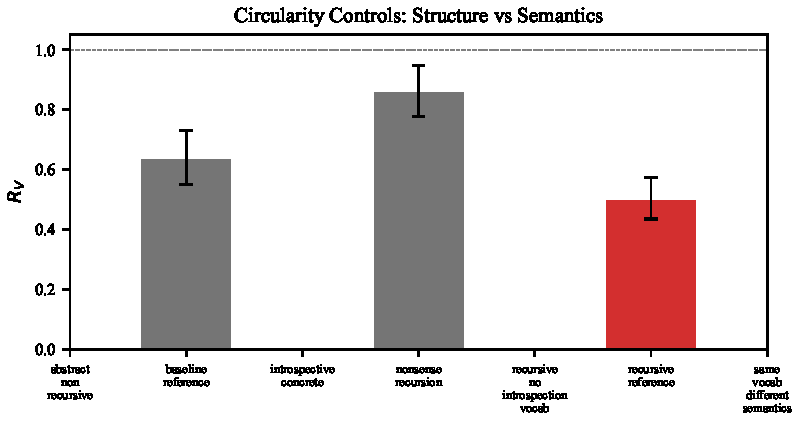
\includegraphics[width=0.72\linewidth]{fig10_circularity_controls.pdf}
\caption{\textbf{Double dissociation: $\RV$ distributions by condition.}
         Combined: $\dcohen = -2.63$ vs.\ baseline.
         Structure only: $\dcohen = -0.062$ (NS).
         Vocab only: $\dcohen = +0.614$ (NS; slight expansion).
         Dashed line: detection threshold ($\RV = 0.737$).}
\label{fig:dissociation}
\end{figure}


%%============================================================
%% SECTION STUBS — CARRY FORWARD FROM v005 WITH REVISIONS
%%============================================================

\draftnote{SECTION 4 (Cross-Architecture): Update signed Cohen's d throughout; remove $|$d$|$ notation.
Note: OPT-6.7B and GPT-2 XL show sign reversal between pipelines (cross-arch: negative;
power-up: positive). Report honestly or flag as pending P0 canonical pipeline experiment
(scripts/p0\_canonical\_pipeline.py). The sign reversal may be a float16 artifact; P0 runs bfloat16.
4 clean Tier 1 models: Mistral, Qwen2.5-7B, Mixtral-8x7B, Gemma-2-9B.}

\draftnote{SECTION 5 (Causal Analysis — MAJOR REVISION): Remove sufficiency claim entirely.
Corrected framing: NECESSITY established (dual-layer ablation h=1.31, BT+ART 56\%->3.7\%).
NOTE: 27.7\% was factual error, already fixed in v005. SUFFICIENCY NOT ESTABLISHED: geometry injection does not
reliably induce recursive behavior. Add path patching: V-proj max $|$d$|$=0.22 (negligible),
early residual stream L4 d=1.96 — this is the causal site. The KV-cache OR=13.96 result transfers
semantic context, not geometry alone; do not conflate with geometric sufficiency.}

\draftnote{SECTIONS 6–9: Carry forward from v005 with minimal changes.
Fix: replace $|$d$|$ notation with signed d throughout Section 8.
Keep: AUROC=0.909, content-vs-intent finding (genuine vs deceptive d=-0.06, NS).
Keep: full head sweep (606/1024 heads significant).}

\draftnote{SECTION 10 (Discussion): Carry forward the ``Why contraction?'' paragraph.
Add one paragraph on the signature-vs-mechanism distinction and its relation to the
early-residual-stream causal result.}


%%============================================================
%% REFERENCES
%%============================================================
\bibliographystyle{plainnat}
\bibliography{references}

\end{document}
